\documentclass[tikz,border=10pt]{standalone}
\usepackage{amsmath}
\usepackage{amssymb}
\usepackage[T1]{fontenc}
\usetikzlibrary{calc,angles,quotes,through,intersections,arrows.meta}

% ===== Farben =====
\definecolor{tri}{RGB}{200,40,40}
\definecolor{ornge}{RGB}{230,120,60}
\colorlet{lgray}{black!42}

\begin{document}
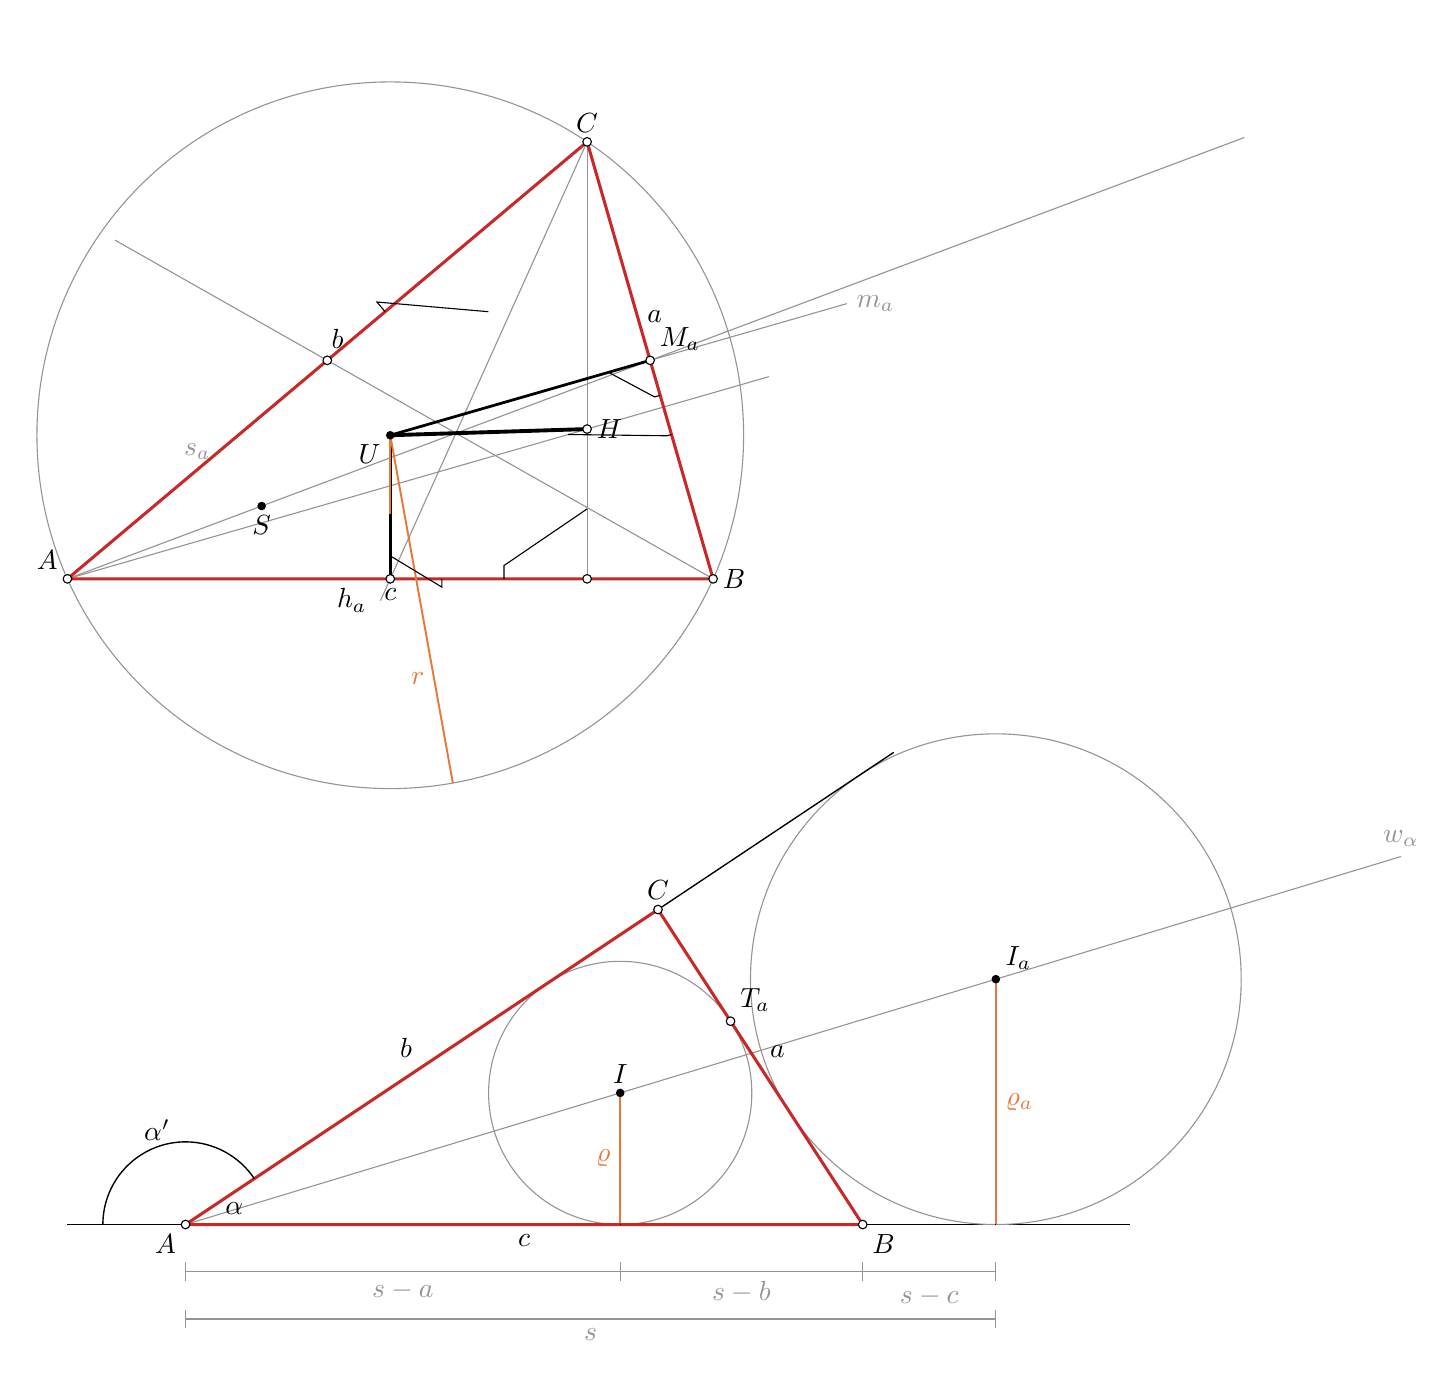
\begin{tikzpicture}[
  >=stealth,
  side/.style={tri,line width=1.1pt},
  aux/.style={lgray,line width=0.4pt},
  rad/.style={ornge,line width=0.7pt},
  dot/.style={circle,fill=black,inner sep=1.1pt},
  hdot/.style={circle,draw=black,fill=white,inner sep=1.1pt,line width=0.4pt},
]

%=====================================================================
% ============  DREIECK 1: Merkwürdige Punkte / Umkreis  =============
%=====================================================================
\begin{scope}
  \coordinate (A) at (0,0);
  \coordinate (B) at (8.2,0);
  \coordinate (C) at (6.6,5.55);

  % Seitenmittelpunkte
  \coordinate (Ma) at ($(B)!0.5!(C)$);
  \coordinate (Mb) at ($(A)!0.5!(C)$);
  \coordinate (Mc) at ($(A)!0.5!(B)$);

  % Umkreismittelpunkt U: Schnitt der Mittelsenkrechten von AB und BC
  \path[name path=msAB] ($(Mc)+(0,-1)$)--($(Mc)+(0,7)$);
  \path[name path=msBC] ($(Ma)!-6cm!90:(B)$)--($(Ma)!6cm!90:(B)$);
  \path[name intersections={of=msAB and msBC, by=U}];

  % Lotfußpunkte
  \coordinate (Hc) at ($(A)!(C)!(B)$);
  \coordinate (Ha) at ($(B)!(A)!(C)$);
  \coordinate (Hb) at ($(A)!(B)!(C)$);

  % Höhenschnittpunkt H
  \coordinate (H) at (intersection of C--Hc and A--Ha);

  % Schwerpunkt S
  \coordinate (S) at ($(A)!0.3333!(Ma)$);

  % Umkreisradius-Strahl nach unten (endet auf dem Kreis)
  \path let \p1=(U) in
    coordinate (Rdir) at ($(U)+(0.18,-1)$)
    coordinate (Rend) at ($(U)!{veclen(\x1,\y1)}!(Rdir)$);

  % Umkreis
  \node[draw=lgray,line width=0.4pt,circle through={(A)}] at (U) {};

  % Hilfslinien
  \draw[aux] (A)--($(A)!2.02!(Ma)$);
  \draw[aux] (B)--($(B)!1.55!(Mb)$);
  \draw[aux] (C)--($(C)!1.05!(Mc)$);
  \draw[aux] ($(Ma)!-2cm!90:(B)$)--($(Ma)!2.6cm!90:(B)$);
  \draw[aux] (C)--(Hc);
  \draw[aux] (A)--($(A)!1.35!(H)$);

  % Seiten
  \draw[side] (A)--(B)--(C)--cycle;

  % Euler-Strecke & Verbindungen zu Mittelpunkten
  \draw[line width=1.4pt] (U)--(H);
  \draw[line width=1.0pt] (U)--(Ma);
  \draw[line width=1.0pt] (U)--(Mc);

  % Radius r (U zum Umkreis, nach unten-rechts)
  \draw[rad] (U)--($(U)!1cm!(Mc)$);
  \draw[rad,line width=0.7pt] (U)--(Rend);

  % Rechtwinkel-Marker
  \def\rasz{0.16}
  \foreach \P/\Q/\R in {Ma/B/U, Mc/B/U, Hc/A/C, Ha/B/A, Hb/A/B}{
    \draw[black,line width=0.4pt]
      ($(\P)!\rasz!(\Q)$) -- ($($(\P)!\rasz!(\Q)$)!\rasz!90:(\P)$)
      -- ($(\P)!\rasz!(\R)$);
  }

  % Punkte
  \node[hdot] at (A){}; \node[hdot] at (B){}; \node[hdot] at (C){};
  \node[hdot] at (Ma){}; \node[hdot] at (Mb){}; \node[hdot] at (Mc){};
  \node[hdot] at (Hc){};
  \node[dot] at (U){}; \node[hdot] at (H){}; \node[dot] at (S){};

  % Beschriftungen
  \node[above left] at (A){$A$};
  \node[right]      at (B){$B$};
  \node[above]      at (C){$C$};
  \node[left]       at ($(A)!0.55!(C)$){$b$};
  \node[right]      at ($(B)!0.6!(C)$){$a$};
  \node[below]      at ($(A)!0.5!(B)$){$c$};
  \node[above right]at (Ma){$M_a$};
  \node[below left] at (U){$U$};
  \node[right]      at (H){$H$};
  \node[below]      at (S){$S$};
  \node[lgray,right] at ($(Ma)!2.6cm!90:(B)$){$m_a$};
  \node[lgray,above] at ($(A)!0.5!(Mb)$){$s_a$};
  \node[below right] at ($(A)!0.5!(Hc)$){$h_a$};
  \node[ornge,left]  at ($(U)!0.7!(Rend)$){$r$};
\end{scope}


%=====================================================================
% =========  DREIECK 2: Inkreis & Ankreis a, w_alpha  ===============
%=====================================================================
\begin{scope}[shift={(1.5,-8.2)}]
  % ---- Eckpunkte (frei wählbar) ----
  \def\Ax{0}\def\Ay{0}
  \def\Bx{8.6}\def\By{0}
  \def\Cx{6}\def\Cy{4}
  \coordinate (A2) at (\Ax,\Ay);
  \coordinate (B2) at (\Bx,\By);
  \coordinate (C2) at (\Cx,\Cy);

  % ---- Seitenlängen aus den Koordinaten (robust gegenüber Verschiebung von C) ----
  \pgfmathsetmacro{\la}{veclen(\Bx-\Cx, \By-\Cy)}   % a = |BC|
  \pgfmathsetmacro{\lb}{veclen(\Ax-\Cx, \Ay-\Cy)}   % b = |CA|
  \pgfmathsetmacro{\lc}{veclen(\Ax-\Bx, \Ay-\By)}   % c = |AB|
  \pgfmathsetmacro{\ssm}{(\la+\lb+\lc)/2}           % s

  % ---- Inkreismittelpunkt I (baryzentrisch a:b:c) ----
  \coordinate (I) at
    ({(\la*\Ax + \lb*\Bx + \lc*\Cx)/(\la+\lb+\lc)},
     {(\la*\Ay + \lb*\By + \lc*\Cy)/(\la+\lb+\lc)});
  \coordinate (Ifoot) at ($(A2)!(I)!(B2)$);

  % Berührpunkt T_a
  \coordinate (Ta) at ($(B2)!{(\ssm-\lb)/\la}!(C2)$);

  % Ankreismittelpunkt
  \coordinate (Ia) at ($(A2)!{\ssm/(\ssm-\la)}!(I)$);
  \coordinate (Iafoot) at ($(A2)!(Ia)!(B2)$);

  % Grundgerade
  \draw[black,line width=0.5pt] (-1.5,0)--(12.0,0);

  % Winkelhalbierende
  \draw[aux] (A2)--($(A2)!1.5!(Ia)$);

  % Inkreis & Ankreis
  \node[draw=lgray,line width=0.4pt,circle through={(Ifoot)}] at (I) {};
  \node[draw=lgray,line width=0.4pt,circle through={(Iafoot)}] at (Ia) {};

  % ---- Verlängerungen als Tangenten am Ankreis ----
  % Tangente entlang Seite a, Gesamtlänge = a (deckungsgleich mit Seite a)
  \draw[aux] (C2)--(B2);
  % Strahl von A durch C (Seite b verlängert) bis zur oberen Tangente
  \draw[black,line width=0.5pt] (A2)--($(A2)!{(\lb+3.6)/\lb}!(C2)$);

  % Radien
  \draw[rad] (I)--(Ifoot);
  \draw[rad] (Ia)--(Iafoot);

  % Seiten
  \draw[side] (A2)--(B2)--(C2)--cycle;

  % ---- Innenwinkel alpha bei A (Richtung A->C) ----
  \pgfmathsetmacro{\angA}{atan2(\Cy-\Ay, \Cx-\Ax)}
  % Außenwinkelbogen alpha' (von der negativen x-Achse, 180°, bis zur Seite AC)
  \draw[black,line width=0.5pt]
     ($(A2)+(-1.05,0)$) arc[start angle=180, end angle=\angA, radius=1.05cm];

  % Rechtwinkel-Marker (Grundlinie x Radius): echtes Quadrat
  \def\rb{0.16}
  \foreach \P/\Q/\R/\tag in {Ifoot/B2/I/one, Iafoot/B2/Ia/two}{
    \path let \p1=($(\Q)-(\P)$), \p2=($(\R)-(\P)$),
              \n1={veclen(\x1,\y1)}, \n2={veclen(\x2,\y2)}
      in
      coordinate (mq\tag) at ($(\P)+\rb*(\x1/\n1,\y1/\n1)$)
      coordinate (mr\tag) at ($(\P)+\rb*(\x2/\n2,\y2/\n2)$)
      coordinate (mc\tag) at ($(\P)+\rb*(\x1/\n1,\y1/\n1)+\rb*(\x2/\n2,\y2/\n2)$);
    \draw[black,line width=0.4pt] (mq\tag) -- (mc\tag) -- (mr\tag);
  }

  % Maßlinien
  \def\yI{-0.6}\def\yII{-1.2}
  \foreach \p in {A2,Ifoot,B2,Iafoot}{
    \draw[lgray,line width=0.4pt] ($(\p)+(0,\yI+0.12)$)--($(\p)+(0,\yI-0.12)$);
  }
  \draw[lgray,line width=0.4pt] ($(A2)+(0,\yI)$)--($(Ifoot)+(0,\yI)$)
    node[midway,below]{$s-a$};
  \draw[lgray,line width=0.4pt] ($(Ifoot)+(0,\yI)$)--($(B2)+(0,\yI)$)
    node[midway,below]{$s-b$};
  \draw[lgray,line width=0.4pt] ($(B2)+(0,\yI)$)--($(Iafoot)+(0,\yI)$)
    node[midway,below=2pt]{$s-c$};
  \foreach \p in {A2,Iafoot}{
    \draw[lgray,line width=0.4pt] ($(\p)+(0,\yII+0.12)$)--($(\p)+(0,\yII-0.12)$);
  }
  \draw[lgray,line width=0.4pt] ($(A2)+(0,\yII)$)--($(Iafoot)+(0,\yII)$)
    node[midway,below]{$s$};

  % Punkte
  \node[hdot] at (A2){}; \node[hdot] at (B2){}; \node[hdot] at (C2){};
  \node[dot] at (I){}; \node[dot] at (Ia){}; \node[hdot] at (Ta){};

  % Beschriftungen
  \node[below left]  at (A2){$A$};
  \node[below right] at (B2){$B$};
  \node[above]       at (C2){$C$};
  \node[above left]  at ($(A2)!0.5!(C2)$){$b$};
  \node[above right] at ($(B2)!0.5!(C2)$){$a$};
  \node[below]       at ($(A2)!0.5!(B2)$){$c$};
  \node[above]       at (I){$I$};
  \node[above right] at (Ia){$I_a$};
  \node[above right] at (Ta){$T_a$};
  \node[ornge,left]  at ($(I)!0.5!(Ifoot)$){$\varrho$};
  \node[ornge,right] at ($(Ia)!0.5!(Iafoot)$){$\varrho_a$};
  \node at ($(A2)+(0.62,0.2)$){$\alpha$};
  \node at ($(A2)+({1.25*cos((180+\angA)/2)},{1.25*sin((180+\angA)/2)})$){$\alpha'$};
  \node[lgray,above] at ($(A2)!1.5!(Ia)$){$w_\alpha$};
\end{scope}

\end{tikzpicture}
\end{document}
